\documentclass[10pt,a4paper]{report}
\usepackage[utf8]{inputenc}
\usepackage[spanish]{babel}
\usepackage{amsmath}
\usepackage{amsfonts}
\usepackage{amssymb}
\usepackage{graphicx}
\usepackage{cite}
\usepackage{xcolor}
\usepackage{url}

 
\author{José Carbonell Caballero}
\title{Identificación y priorización de genes candidatos en enfermedades hereditarias: un estudio basado en redes génicas}
%
%\renewcommand{\chapter}[1]{ 
%
%\begin{flushright}
%
%	\begin{LARGE}
%	   \thechapter{}
%	\end{LARGE}	
%	\\
%	\line(1,0){250}
%	\\
%	\begin{LARGE}
%	#1
%	\end{LARGE}
%
%\end{flushright}
%	
%\medskip
%	
%}

\makeatletter
\def\thickhrule{\leavevmode \leaders \hrule height .5pt \hfill \kern \z@}
\def\position{\centering}
%% Note the difference between the commands the one is 
%% make and the other one is makes
\renewcommand\@makechapterhead[1]{%
  \vspace*{10\p@}%
  {\parindent \z@ \position \reset@font
       % {\Huge \scshape  \thechapter }
        \par\nobreak
        \vspace*{5\p@}%
        \interlinepenalty\@M
        \thickhrule
        \par\nobreak
        \vspace*{2\p@}%
            % hacken om nummer 0 niet te weergeven 
        \noindent
        \parbox{\linewidth}{\raggedleft\Huge \bfseries 
          \ifnum\thechapter>0 \thechapter\space\fi #1}\par\nobreak}
        \par\nobreak
        \vspace*{2\p@}%
        \noindent
        \thickhrule
    \vskip 50\p@
  }

%% This uses makes

\def\@makeschapterhead#1{%
  \vspace*{10\p@}%
  {\parindent \z@ \position \reset@font
        %{\Huge \scshape \vphantom{\thechapter}}
        \par\nobreak
        \vspace*{5\p@}%
        \interlinepenalty\@M
        \thickhrule
        \par\nobreak
        \vspace*{2\p@}%
        \noindent
        \parbox{\linewidth}{\raggedleft\Huge \bfseries #1}
        \par\nobreak
        \vspace*{2\p@}%
        \thickhrule
    \vskip 50\p@
  }}
\makeatother



\begin{document}



\maketitle

\pagebreak

\begin{abstract}
Esto será el abstract...
\end{abstract}

\pagebreak

\tableofcontents

\pagebreak

\bibliographystyle{unsrt}



\chapter{Introducción}


\section{Biología molecular y computacional}

% Biología molecular

\subsection{Los inicios de la biología molecular}

La biología molecular surge como una disciplina propia a raíz del descubrimiento de la doble hélice de ADN por parte de los investigadores James D. Watson y Francis Crick en 1953 \cite{watsonycrick}, descubrimiento por el cual fueron galardonados, junto a Maurice Wilkins, con el premio Nobel de medicina en 1962. Este hallazgo, que pasó desapercibido en un primer momento, fue el inicio de una serie de trabajos que permitieron describir como el ADN codifica en su interior las instrucciones necesarias para el funcionamiento de las células. Se descubrió que los aminoácidos se codificaban en grupos de 3 nucleótidos y que una secuencia de estos, formaba una proteína, la cual es la encargada directa de ejecutar las instrucciones contenidas en una determinada porción del ADN. A partir de ese momento, la biología molecular crece como una rama esencial de la biología y gracias a la influencia de otras ramas como la bioquímica, surge con un carácter marcadamente cuantitativo, dentro de una ciencia más acostumbrada a la descripción que a la medición.

\medskip

En términos generales, la biología molecular se define como la parte de la biología encargada de estudiar los procesos celulares que ocurren a escala molecular. Estos procesos abarcan todos los mecanismos necesarios para que las células puedan funcionar correctamente, llevando a cabo todas sus funciones vitales con normalidad. Se trata de mecanismos generales que ocurren en todos los organismos conocidos, aunque por supuesto, con diferencias específicas en función del tipo celular.

\medskip

La biología molecular nos permite comprender como funcionan las células y que mecanismos son esenciales para preservar la vida. Es de especial interés la composición de las diferentes formas de material genético (ARN o ADN) y los elementos moleculares que intervienen en su síntesis y regulación. Cinco años después del descubrimiento de la doble hélice, Francis Crick formula lo que se conoce como \emph{dogma central de la biología molecular}. El dogma básicamente describe como la porción de ADN correspondiente a un gen se copia (o transcribe) en forma de ARN mensajero y como este sale del núcleo y acaba siendo traducido a una proteína que llevará a cabo la función del gen. A pesar de que con el tiempo se ha demostrado que el dogma central no refleja con exactitud lo que ocurre a nivel celular, ha servido para ilustrar de forma intuitiva el ciclo de vida de los genes y como son capaces de llevar a cabo su función en la célula (\ref{fig:dogma}).

\begin{figure}
\centering
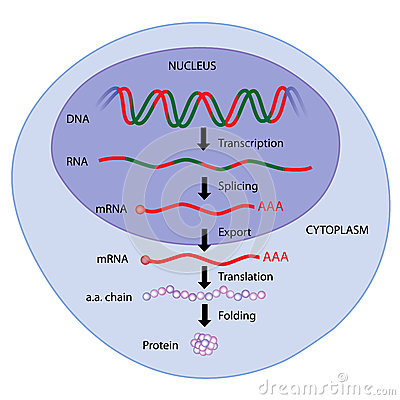
\includegraphics[scale=0.5]{images/dogma_central.jpg}
\caption{Dogma central de la biología molecular}
\label{fig:dogma}
\end{figure}


\subsection{Biología computacional}

Desde los descubrimientos de Watson y Crick, la biología molecular ha crecido de la mano de un sinfín de tecnologías que le han permitido abordar de forma cuantitativa el estudio de fenómenos a escala molecular. Desde el microscopio hasta los modernos secuenciadores, todos los descubrimientos han estado asentados sobre una base tecnológica muy fuerte, de la que han carecido otras áreas de la biología. 

\medskip
Una de las ramas tecnológicas que más ha evolucionado y aportado a la biología molecular en los últimos 30 años ha sido la informática. Esta rama ha  permitido procesar y almacenar de forma ordenada cantidades enormes de datos en tiempos de cómputo razonables. A la aplicación de la informática a la biología y su unión a otras disciplinas como la estadística o las matemáticas, se le denominó biología computacional.
  
\medskip 
La biología computacional, también denominada bioinformática, es una disciplina en la que, a partir de la combinación de modelos, algoritmos y computadores, es posible abordar la resolución de problemas de tipo biológico. Los problemas más característicos afrontados en el pasado mediante la biología computacional han estado relacionados con el alineamiento de secuencias, lo que ha permitido, entre otras cosas, construir árboles filogenéticos que describen como evolucionan y se relacionan las especies cercanas con sus ancestros comunes.

\medskip
En los últimos años, el volumen de datos aportados por la biología molecular ha crecido de forma considerable, lo que ha generado una gran dependencia a nivel informático que ha obligado a la incorporación de procedimientos y herramientas informáticas que permiten automatizar ciertos procesos casi cotidianos.  

\medskip
Entre los logros más importantes de la biología molecular y computacional destaca el Proyecto Genoma Humano \cite{pgh}, encargado de la determinación total de la secuencia de nucleótidos que compone el genoma humano. Esta tarea requirió más de 13 años de trabajo y una inversión superior a 280.000 millones de dólares, aportados mayoritariamente por los gobiernos de Gran Bretaña y Estados Unidos. La descripción de la secuencia del genoma humano y la localización de los genes tuvo una gran relevancia en los ámbitos de la biomedicina y la genética clínica, permitiendo arrojar luz sobre las bases moleculares de algunas enfermedades hereditarias.

\section{Enfermedades de origen genético}

\subsubsection{Enfermedades hereditarias}

Las enfermedades de origen genético son síndromes donde un error en la maquinaria de síntesis de proteínas provoca un comportamiento anómalo de las células y como consecuencia, la aparición de una enfermedad. Típicamente, su origen viene determinado por una mutación o variación estructural nociva en uno o varios genes, provocando un daño en cadena.

\medskip

Cuando la enfermedad está causada por un único gen, decimos que es monogénica o mendeliana (en honor a Gregor Mendel). Ejemplos de enfermedades monogénicas son la fibrosis quística (causada por el gen \textit{CFTR})\cite{fq}, la enfermedad Huntington (causada por el gen HTT)\cite{huntington}, o la Hemofilia de tipo A (causada por el gen F8)\cite{hemofilia}. Por el contrario, cuando la enfermedad está causada por la combinación de varios genes mutados, entonces decimos que es multigénica. Las enfermedades multigénicas son mucho más frecuentes que las monogénicas, y engloban a la mayoría de enfermedades crónicas como la hipertensión, la obesidad, o síndromes complejos como el alzheimer o la esquizofrénia. 

\medskip
Cuando la enfermedad es de carácter familiar, entonces decimos que es hereditaria. En este caso, la mutación o mutaciones nocivas se segregan de padres a hijos. Sin embargo, no todos los individuos portadores acabarán desarrollando la enfermedad, depende del modelo de herencia de la enfermedad. 

\subsubsection{Estructura genómica y modelos de enfermedad}

Los humanos disponemos de un genoma redundante compuesto por 23 pares de cromosomas, lo que significa a efectos prácticos (y a excepción de los cromosomas sexuales) que disponemos de dos copias iguales de cada gen, donde una copia vendrá proporcionada por vía paterna y la otra por vía materna. 

\medskip
*** figura cromosomas en la célula punto de recombinarse

\medskip
Esta duplicidad génica tiene efectos beneficiosos, tanto sobre el individuo como sobre la especie, ya que genera (por combinación) biodiversidad, haciéndonos más resistentes a enfermedades. Sin embargo, también tiene efectos funcionales ya que, cada parental dispone de variaciones estructurales y mutaciones propias que generan pequeñas diferencias entre las dos copias génicas que recibe cada descendiente. 

\medskip
Cuando una mutación está presente sólo en una copia, entonces decimos que se presenta en heterocigosis, sin embargo cuando la mutación es compartida por ambas copias, es decir, ambos parentales disponían de ella, entonces decimos que está presente en homocigosis. 

\medskip
Cuando una enfermedad hereditaria muestra una herencia de tipo recesivo, significa que será necesario disponer de una mutación nociva en ambas copias del gen para acabar desarrollando la enfermedad, lo que generalmente estará asociado a una pérdida de función del gen, ya que ninguna de sus proteínas acabará siendo funcional. Sin embargo, cuando la herencia de la enfermedad es de tipo dominante, entonces significa que, o bien, la copia intacta no es capaz de compensar la ausencia de la copia mutada, o bien la proteína mutada dispondrá de una nueva función que resultará nociva para la célula.  

\medskip
Comprender como funcionan los distintos modelos de enfermedad resulta absolutamente fundamental, ya que nos permite entender las bases moleculares de las enfermedades y por consiguiente, avanzar en su prevención y cura. Además, nos permite ser mucho más eficientes a la hora de buscar genes que puedan estar implicados en una enfermedad con un origen genético total o parcialmente desconocido. El problema se complica cuando las variaciones genómicas no son responsables en su totalidad del inicio de la enfermedad. En este caso, las condiciones ambientales (como los hábitos alimenticios o el clima) explican un porcentaje significativo del riesgo a desarrollar la enfermedad. Existen enfermedades como el cáncer de pulmón, donde los hábitos (como ser fumador) juegan un papel decisivo en su riesgo y proliferación, y otras enfermedades, principalmente monogénicas, donde presentar ciertas variaciones estructurales asegura una penetrancia casi total, con independencia de los hábitos del individuo.

\medskip
Dentro del estudio de enfermedades hereditarias, es de especial interés el estudio de enfermedades raras. Las enfermedades raras, o también conocidas como huérfanas, son aquellas que tienen una baja incidencia en la población (inferior a 5 de cada 10.000 individuos) y por su condición de baja prevalencia, son sometidas a menores inversiones por parte de capital público y privado. Existen más de 7000 enfermedades raras descritas por la OMS y se estima que afectan al 7\% de la población mundial (sólo en España afectan a más de 3 millones de personas). Este tipo de síndromes se benefician claramente de las estrategías de secuenciación de genoma completo, ya que de otra forma, serían necesarios costosos estudios previos que focalizaran el origen de la enfermedad sobre un grupo reducido de genes candidatos.

\medskip
Panorama mundial /penetrancia/ ***

\subsubsection{Repositorios de polimorfismos y mutaciones}

\medskip
1000 genomas: mutaciones en población sana ***

\section{Secuenciación de ADN}

\subsection{La secuenciación del genoma}

La secuenciación del ADN nos permite conocer el orden específico de los nucleótidos en el genoma de un individuo, lo que posteriormente facilita la identificación y localización de los genes. Comparando la secuencia obtenida con una secuencia de referencia es posible determinar aquellas diferencias o variaciones estructurales que presenta un individuo y que podrían ser susceptibles de haber causado o causar una enfermedad en el futuro. La construcción de un genoma de referencia con el que comparar ya supone de por sí un reto tecnológico importante que ha sido llevado a cabo en la última década. Además, el genoma de referencia constituye una plantilla sana con la que comparar y definir la normalidad no es algo sencillo. Esta importante tarea recae sobre un consorcio internacional \cite{GRC} encargado de construir y almacenar la versión oficial del genoma humano, actualizándolo de forma periódica.

\medskip
La secuenciación de genomas o porciones de ADN ha sido llevada a cabo por medio de diferentes procedimientos a lo largo de los últimos 50 años. Los métodos implementados han permitido determinar con fiabilidad la secuencia de nucleótidos correspondiente a un fragmento de material genético. Todos los métodos han mostrado tasas de error cuantificables y parámetros críticos como su complejidad, facilidad de ejecución, velocidad de secuenciación o coste económico, los cuales han sido claves para su evolución y adopción por parte de los investigadores. 

\medskip
Uno de los principales handicaps producidos por el desarrollo de tecnología heterogénea es que cada método de secuenciación ha venido acompañado de su propia base científica y de numerosas herramientas y métodos estadísticos de análisis específicos, lo que ha requerido un reaprendizaje de las herramientas de trabajo por parte de los investigadores. Este hecho ha tenido especial incidencia en los últimos años ya que cada tecnología ha dado lugar a una batería de herramientas informáticas de análisis y de algoritmos encargados de resolver problemas específicos de cada tecnología. 

\medskip
A continuación, se enumeran tres de las metodologías de secuenciación más empleados en la biología molecular. Cabe destacar que a pesar de mostrar una cronología clara, todos los métodos son actualmente vigentes y es habitual verlos coexistir en proyectos genómicos, donde cada tecnología es usada en su ámbito adecuado. 


\subsection{Secuenciación por \emph{Sanger}}

El método de secuenciación más empleado en las últimas décadas ha sido el denominado método \emph{Sanger} \cite{sanger}, en honor a su creador Frederick Sanger. Sanger, el cual es una de las 4 personas que han recibido un premio Nobel dos veces en su vida, fue capaz de demostrar que las proteínas tienen una estructura específica y que esta es fundamental para su función. Para ello, consiguió en 1955 determinar la secuencia de aminoácidos de la insulina y desarrolló un método con el que obtuvo un perfil específico de su estructura \cite{sanger_estructura}. Este trabajo le permitió obtener su primer nobel de química en 1958. Años más tarde (en 1975) desarrolla formalmente su método de secuenciación \cite{Sanger1977}, el cual, a partir de dideoxinucleótidos, un gel de agarosa y la aplicación de electroforesis fue capaz de obtener un patrón de bandas a partir del cual es posible deducir la secuencia subyacente de nucleótidos. 

\medskip
Con este método, Sanger secuenció al bacteriófago A4, que se convirtió en el primer organismo cuyo genoma fue secuenciado de forma completa. Los trabajos de Sanger fueron fundamentales en la consecución del \emph{Proyecto Genoma Humano} y en otros ambiciosos proyectos de secuenciación posteriores, gracias a lo cual fue galardonado con su segundo nobel de química en 1980. 

\subsection{Chips de ADN}

A pesar de los importantes avances obtenidos mediante la secuenciación por Sanger, ha sido necesario evolucionar a formas más rápidas y automáticas de secuenciación que dejaran atrás algunas limitaciones técnicas como la secuenciación de largas cadenas de ADN. Con una perspectiva sistémica, se ha evolucionado hacia métodos de secuenciación que son capaces de obtener información simultanea de miles de genes. 

\medskip
Una de las tecnologías más populares surgidas en la última década han sido los chips de ADN, los cuales, gracias su buena relación coste/prestaciones se extendieron rápidamente a la gran mayoría de estudios biomédicos con una componente genómica importante.

\medskip
Un chip de ADN se compone de una matriz de sondas (o pocillos), donde cada elemento es capaz de medir información concreta acerca de un gen. Los chips más empleados han sido los de expresión génica. Estos, recogen en cada pocillo una porción de la secuencia complementaria de cada gen, a partir de la cual son capaces de obtener una medida proporcional a la abundancia de ARN mensajeros y por tanto de la expresión de los genes. 

*** figura microarrays

\medskip
Otros chips ampliamente extendidos, han sido los chips de genotipado. En este caso, el chip se encarga de testar la presencia de una cantidad enorme de polimorfismo en la secuencia de los genes, que actuan sobre marcadores genómicos asociados a enfermedades.

\medskip
Si bien, los chips de ADN no han constituido una tecnología capaz de obtener la secuencia precisa de nucleótidos de cada gen, sí han servido de forma eficiente y barata para la determinación algunas características esenciales relacionadas con la dinámicas de los genes.

\subsection{Ultrasecuenciadores o técnicas de secuenciación masiva}

Los avances de la última década han permitido el desarrollo de técnicas de secuenciación másiva a un coste muy bajo. Se trata de tecnologías que permiten procesar y secuenciar simultáneamente millones de fragmentos de ADN. Son las llamadas tecnologías de ultrasecuenciación o secuenciación másiva y son capaces de secuenciar un genoma completo en aproximadamente una semana, con un coste inferior a 20.000 dolares, algo que hace 15 años habría sido difícil de imaginar. Lógicamente, estas técnicas han revolucionado la genómica computacional, dirigiendo los estudios hacia una perspectiva más genómica que génica.

\medskip
A pesar de sus numerosas prestaciones, los técnicas de secuenciación másiva también muestran algunas limitaciones importantes. La más destacada reside en la longitud máxima que los aparatos son capaces de secuenciar. Actualmente, los secuenciadores son capaces de obtener fragmentos de entre 50 y 500 nucleótidos, lo cual, comparado con técnicas clásicas como la secuenciación por Sanger, resulta muy pobre. Además, los fragmentos de ADN secuenciados tienen que volver a ser reposicionados sobre el ADN para poder reconstruir el genoma completo de la muestra y los secuenciadores no aportan ningún tipo de información a este respecto. Por esta razón, es necesario realizar un paso de computado adicional denominado \emph{mapeo} donde cada fragmento secuenciado se compara con un genoma de referencia. Algunos parámetros, como la longitud del fragmento, serán claves para la fiabilidad del mapeo, ya que, a menor tamaño, más probable será encontrar la misma secuencia de nucleótidos en varios puntos del genoma. 

\medskip
Otra limitación importante reside en la tasa de error obtenida durante la determinación de la secuencia de nucleótidos, la cual es superior al resto de técnicas de secuenciación. Por esta razón, es habitual realizar un análisis estadístico a partir de datos de ultrasecuenciación, complementados con una fase de validación posterior realizada por el método \emph{Sanger}.

\medskip
A pesar de todo, los ultrasecuenciadores constituyen una tecnología más que prometedora que aporta un enfoque genómico muy eficiente en el estudio de aquellas enfermedades donde los genes causantes de la enfermedad son desconocidos


\section{Identificación de genes candidatos}


\subsection{Regiones de interés}

Los genes constituyen únicamente el 5\% del genoma, el resto, antaño considerado como ADN basura [***], tiene una función todavía desconocida, que en algunas ocasiones estará relacionada con aspectos más estructurales que funcionales en la molécula de ADN. A su vez, los genes tienen en su interior cierto grado de estructura. Poseen porciones que serán codificadas directamente a proteínas, llamadas exones o regiones codificantes, pero también poseen otras regiones dedicadas al control de su expresión, e incluso otras regiones, denominadas intrones, implicadas en la formación de las diferentes isoformas del gen.

\medskip
\begin{figure}
\centering
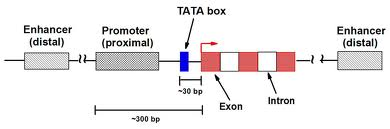
\includegraphics[scale=1]{images/estructura_gen.jpeg} 
\caption{Estructura de un gen}
\end{figure}

\medskip
Debido a la estructura y funcionamiento del genoma, se considera mucho más probable encontrar una mutación causante de enfermedad dentro de una zona codificante, ya que esta produciría un cambio directo sobre las proteínas generadas y por consiguiente, un comportamiento anómalo. Esta circunstancia produce que en la práctica no se realice una secuenciación orientada a genoma completo, por el contrario, se recurre a kits especiales de secuenciación que cubren únicamente las regiones codificantes de los genes. Esta reducción en el área de búsqueda, que puede tener implicaciones serias en casos donde la mutación nociva no afecta a una zona codificante sino a una zona reguladora, permite en la práctica trabajar sólo con el un 2\% del total del genoma, lo cual aporta grandes beneficios para toda la fase de procesamiento, almacenamiento y análisis que ocurre después de la secuenciación, consiguiendo un aprovechamiento máximo de los recursos económicos disponibles dentro de un proyecto de investigación. 

\subsection{Estudio caso/control}

El protocolo de selección de genes candidatos se realiza a partir de un estudio caso/control. En este caso, se trata de identificar a aquellos genes mutados que podrían tener una relación directa con la enfermedad. Como es habitual, el grupo de casos está formado por una serie de individuos que comparten el mismo síndrome, en este caso, de origen genético. 

\medskip
El grupo de casos se acompaña de un grupo de individuos control que nos permite filtrar todas aquellas mutaciones potencialmente nocivas que por estar presentes en población sana no deberían estar relacionadas con el síndrome. 

\medskip
Una vez realizada la secuenciación y el resto de pasos computacionales necesarios, se obtienen todas las mutaciones propias de cada individuo del estudio, descartando a aquellas que no muestren un efecto nocivo probado. Las mutaciones seleccionadas, serán sometidas, generalmente, a un test estadístico de proporciones (como el test exacto de Fisher) que identificará a aquellos candidatos de mayor prevalencia en casos frente a controles. Cabe destacar que este proceso puede realizarse a nivel mutacional, donde todos los individuos enfermos compartirán exactamente el mismo cambio nocivo, o a nivel génico, donde lo importante es identificar al gen mutado, por encima de las variaciones estructurales propias de cada individuo enfermo.

\medskip
Debido a limitaciones relacionadas con el tamaño muestral y otro tipo de sesgos surgidos durante todo el proceso, el gen, o genes causantes serán seleccionados junto a un grupo de genes aleatorios que cumplirán los mismos requisitos y que por tanto no podrán ser filtrados ni separados de estos. Será tarea de estrategias posteriores encontrar argumentos biológicos o técnicos que permitan reducir el número de candidatos y priorizar convenientemente a los que quedan, ya que, los mecanismos de validación posteriores son complejos e incorporan de forma habitual costosos trabajos de laboratorio. El tamaño muestral y otros parámetros de calidad relacionados con la secuenciación condicionarán claramente la talla del conjunto de genes candidatos, aunque otros aspectos relacionados con la fase computacional también podrían tener gran influencia.


\subsection{Reducción y priorización de genes candidatos}

La identificación de los genes implicados en el origen de una enfermedad hereditaria constituye una tarea ardua, con unos requerimientos temporales y económicos considerables, en la que es habitual enfrentarse al estudio detallado de cientos de genes candidatos. En este contexto, es necesario contar con protocolos de priorización (manuales o automáticos) que permitan reducir la lista de candidatos iniciales o priorizar convenientemente a los seleccionados en función de criterios biológicos.

\medskip
El proceso de priorización establece un ranking de genes que estima la relevancia de cada candidato sobre los procesos biológicos que se presuponen clave en la enfermedad de estudio, siendo los mejor priorizados aquellos que serán empleados en los análisis posteriores. Los criterios empleados hasta la fecha para determinar la implicación de un gen sobre una enfermedad son muy amplios. En general, se comienza haciendo uso de la estructura de los individuos del estudio caso/control, para posteriormente, recopilar propiedades inherentes a los genes que describen su relevancia global, y en consecuencia, permite modular las probabilidades a priori de cada candidato propuesto. 

\medskip
La selección de genes candidatos comienza generalmente por la delimitación de aquellas regiones del genoma que podrían contener al gen o genes causantes. Esta tarea se ha llevado a cabo por medio de estudios que relacionan zonas cromosómicas con rangos fenotípicos, o en casos familiares, a partir de la intersección entre las zonas mutadas de uno o varios individuos enfermos con sus parentales también afectados.

\medskip
Desgraciadamente, las técnicas de posicionamiento no consiguen centrar convenientemente el problema sobre una reducida lista de regiones que todavía contenga al gen de la enfermedad. Además, muestran algunas limitaciones claras, especialmente en síndromes de origen regulatorio, donde es difícil delimitar las regiones cromosómicas afectadas, y no tienen en cuenta el plegamiento tridimensional de los cromosomas que provoca que dos genes cercanos en el espacio, aparezcan alejados al tratar la secuencia de ADN como un fragmento lineal. A pesar de todo, constituyen un buen punto de inicio, y permiten filtrar algunas regiones candidatas que sólo aportarían ruido al análisis.

\medskip
El uso de información funcional acerca de los genes permite establecer de forma eficiente criterios cuantitativos y cualitativos de \emph{culpabilidad} sobre los candidatos. Las bases de datos con información biológica describen cómo los genes intervienen en rutas metabólicas y de señalización \cite{kegg}, qué funciones biológicas desempeñan en la célula y en qué compartimentos\cite{go}, qué mutaciones han sido descritas previamente \cite{dbsnp} y en qué enfermedades han sido implicadas \cite{hgmd}, así como otro tipo de anotaciones biológicas que pueden tener gran relevancia a la hora de obtener un perfil específico de cada gen. 

\medskip
La información cubre generalmente las siguientes áreas:

\bigskip
\begin{itemize}{}{}
\item \emph{Redes de interacción proteína-proteína:}\\ Interacciones físicas entre las proteínas generadas por los genes.
\item \emph{Anotaciones funcionales:}\\Funciones biológicas, compartimentos celulares y otros roles asignados a las proteínas.
\item \emph{Rutas metabólicas y de señalización:}\\Diagrama de las diferentes rutas biológicas en las células y su implicación en algunas enfermedades.
\item \emph{Asociación a enfermedades:}\\Asociaciones descritas en la literatura de tipo gen/enfermedad o mutación/enfermedad.
\item \emph{Expresión:}\\Expresión de los genes por tejido o momento del desarrollo.
\item \emph{Conservación:}\\Grado de conservación de la secuencia de nucleótidos entre diferentes especies cercanas.
\item \emph{Redes de regulación:}\\Relaciones entre genes reguladores y regulados.
\item \emph{Minería de textos:}\\Frecuencia de aparición de un gen en publicaciones científicas, junto a otros términos relativos a enfermedades, procesos biológicos u otras entidades de interés.
\end{itemize}

\bigskip
El concepto de priorización computacional, tal y como hoy lo conocemos, fue introducido por primera vez en 2002 por Perez-Iratxeta\cite{perez-iratxeta}. A partir de ese momento, multitud de métodos y algoritmos, en su mayoría de uso libre, han sido desarrollados para llevar a cabo tal tarea \cite{review1,review2,review3}. Los métodos propuestos consiguen clasificar y priorizar de forma automática grandes cantidades de genes, lo que los hace muy adecuados en estudios de genoma completo, especialmente en el estudio de aquellas enfermedades genéticas de origen desconocido y cuando el número de candidatos es grande.

\medskip
En general, la inmensa mayoría de métodos propuestos tratan de recuperar la información disponible sobre aquellos genes que ya se han descrito en la enfermedad, con el fin de establecer un criterio de priorización sobre los nuevos candidatos. El mecanismo habitual consiste en obtener un vector de características sobre los genes de referencia, que posteriormente será empleado para medir el grado de similitud entre cada candidato y los genes conocidos, siendo el gen más similar el de mejor priorización. Esta metodología reposa sobre la idea básica de que aquellos genes de enfermedad que todavía no han sido descritos, deberían tener características funcionales, similares a los genes existentes. 


\medskip
%Es conocido que no todas las mutaciones en genes van a producir los mismos efectos. Hay mutaciones que ni siquiera provocan un cambio de aminoácido en la secuencia proteíca, y %otras que directamente impiden la síntesis de la proteina. 
%Mutaciones sinónimas/no sinónimas, No todas las mutaciones causan los mismos síntomas o la misma intensidad de la enfermedad ***




\subsection{Validación del conjunto final de genes candidatos}

***modelos animales


***grupo de test


\section{Metodologías de priorización en ausencia de genes conocidos}


\medskip
La metodología habitual presenta algunas limitaciones. En primer lugar, es necesario disponer de una lista de genes previamente descritos para la enfermedad de estudio, algo que no siempre ocurre. En estos casos, aquellos procesos biológicos relevantes podrían aportar una lista de genes cercanos con los que establecer una referencia secundaria. Por otro lado, la mayor parte de enfermedades mendelianas, disponen de muy pocos genes descritos, lo que a nivel estadístico, supone un problema importante durante la fase de construcción del perfil.




\chapter{Material y métodos}


\section{Situación inicial: genes candidatos}

La metodología propuesta en el presente trabajo trata de describir como priorizar un conjunto de genes candidatos obtenidos a partir de un típico estudio caso/control. El contexto de aplicación serán las enfermedades hereditarias y se va a plantear una metodología compatible tanto con un estudio de tipo familiar, donde se dispone de 1 o más familias distintas con el mismo síndrome, pero no necesariamente con la misma mutación, como con un estudio de tipo más general, donde los individuos disponibles no tienen parentesco alguno. 

\medskip
Cuando afrontamos un estudio de tipo familiar, los individuos seleccionados, tanto casos como controles, se distribuyen a lo largo de las distintas familias. Si se ha realizado un diseño experimental en condiciones, cada nucleo familiar, dispondrá tanto de sujetos caso, como de sujetos control propios de la familia. La ventaja proporcionada por las estructuras familiares es que a priori se espera que todos los individuos enfermos pertenecientes a la misma familia compartan exactamente el mismo origen, es decir, la misma mutación dañina (heredada de padres a hijos), lo cual sería mucho más difícil de afirmar en el caso de individuos independientes. Esta situación permite reducir drásticamente el número de candidatos finales con sólo realizar una simple intersección entre las mutaciones de los individuos enfermos. Por otro lado, los familiares sanos incluidos en el estudio dispondrán de una capacidad de filtrado mucho mayor, ya que al compartir con sus familiares enfermos una porción de genoma mayor de lo esperable con un control externo, será posible eliminar una cantidad mayor de mutaciones no relacionadas con la enfermedad. Además, dicha potencia aumentará con el grado de parentesco, se calcula que un hermano sano (el cual compartirá el 50\% de su genoma con el hermano enfermo) puede tener una capacidad de filtrado equivalente a cientos de controles externos. La figura xxx muestras las diferencias básicas entre el protocolo inicial de selección de candidatos para un estudio familiar frente a uno más general. Al final, en cualquiera de los dos casos, se dispone de una lista de genes candidatos para cada grupo de individuos independientes. Si el estudio es familiar, dispondremos de una lista de candidatos para cada familia, mientras que en el caso general, cada individuo aportará su lista de genes. 

\section{Metodología general}

\subsection{Esquema general del método}

La metodología propuesta trata de puntuar a cada gen candidato en función del grado de importancia global sobre el total de familias o individuos estudiados. El proceso se podría describir como una especie de intersección entre los candidatos aportados por cada grupo independiente, donde los genes que aparezcan en un mayor número de grupos serán en general los que tienen una probabilidad mayor de ser responsables de la enfermedad de estudio y por tanto, los mejor priorizados. 

\medskip
Una forma sencilla de abordar el problema cuando esperamos que todos los individuos del estudio tengan mutado el mismo gen, sería mediante la intersección directa de las listas de candidatos proporcionadas por cada familia. En un escenario sencillo, esta sería probablemente la metodología más adecuada, ya que, salvo por un error de secuenciación o procesamiento posterior, el gen de la enfermedad estará presente en todas las listas de candidatos obtenidas. Además, al aumentar el número de familias en el estudio se estará aumentando de forma exponencial la fiabilidad del resultado, ya que, se reduce la probabilidad de encontrar un gen que por azar esté presente también en todas las familias. Sin embargo, cuando disponemos de familias o individuos heterogéneos, con el mismo síndrome, pero con genes mutados diferentes, la metodología de intersección directa no sería valida. El problema se agrava al considerar que los errores del protocolo podrían provocar que el gen de la enfermedad no fuera correctamente secuenciado y que por tanto, no apareciera en la lista de candidatos iniciales. En este caso, es necesario aplicar metodologías más sofisticadas que permitan detectar cuando un gen, aun no habiendo sido seleccionado directamente por una familia, presenta interacciones descritas con los genes que sí han sido seleccionados.

\medskip
Se calcula que más de un 15\% de enfermedades mendelianas disponen de más de un gen distinto con capacidad para producir la enfermedad, este porcentaje aumentaría mucho en el caso de las enfermedades complejas. Esto se debe a que, aun teniendo una función claramente definida, generalmente los genes actuan de forma colaborativa para llevar a cabo los distintos procesos biológicos que ocurren en la célula. Los genes se coordinan en rutas metabólicas, rutas de señalización u otro tipo de procesos biológicos donde el grado de coordinación entre las distintas moléculas participantes es muy alto. De esta forma, si un síndrome está causado por el mal funcionamiento de un determinado proceso biológico en la célula, es probable que mutando cualquiera de sus genes importantes, se acabe produciendo el mismo síndrome. Esto nos obliga a adaptar las metodologías de trabajo, y poder recoger así la heterogeneidad presente en un set de individuos seleccionados para un estudio.

\medskip
El proceso de priorización comienza con el reclutamiento de todas las listas de genes candidatos aportadas por los distintos grupos independientes del estudio. Seguidamente, se construye el conjunto global de candidatos a partir de la unión de todos los genes seleccionados por las familias. 
A continuación, se procede a realizar el cómputo del peso, o estadístico de priorización, para cada uno de los genes incluidos en el conjunto global de candidatos. Por último, una vez obtenidos los pesos de cada uno de los genes candidatos, se realiza un ordenamiento de la lista de genes en función del estadístico calculado. De esta forma, los genes que estén en lo alto de la lista serán los mejor priorizados, y por tanto, los primeros a validar.

\medskip
El cómputo del estadístico de priorización para un determinado gen candidato, se realiza básicamente a partir de la suma del peso que tiene el gen en cada una de las familias del estudio. Cuanto mayor sea el peso del gen en las distintas familias, o mayor sea el número de familias en las que el gen esta presente, mejor será su ponderación. Para calcular la relación entre un gen candidato y una familia de estudio, se realiza una evaluación en dos partes: en primer lugar se proporciona un peso inicial en función de si el gen está presente en la lista de candidatos aportada por la familia (equivalente a la que se realizaría con el método de intersección directa) y en un segundo lugar, se añade un segundo término proporcional a la cantidad de interacciones descritas entre el gen candidato y los genes seleccionados por la familia. Esta metodología permite recoger de forma más eficiente el grado de proximidad entre un gen y una familia, lo que a la postre proporciona una priorización más precisa, permitiendo incluso ponderar de forma satisfactoria, genes que no han sido directamente seleccionados por la familia como candidatos. 

\subsection{Estimación del grado de interacción entre genes candidatos y familias}

\medskip
La parte complicada del proceso reside en como calcular y ponderar el grado de interacción entre un gen candidato y el conjunto de genes aportados por una familia. Para ello, en primer lugar, es necesario disponer de una base de datos que recoja el total de interacciones descritas entre los genes. En este caso, se hará uso de diferentes interactomas. Se trata de ficheros que recogen todas las interacciones descritas entre cada par de genes, a partir de los cuales es posible reconstruir fácilmente la red de interacción global de todas las proteínas o genes. Esta red de interacción, donde los nodos son los genes y las aristas sus interacciones, permite, además de recuperar los genes vecinos que interaccionan directamente con un determinado gen, reconstruir totalmente los caminos o secuencias de genes que podríamos emplear para llegar desde un nodo (o gen) de la red a otro. El conjunto total de caminos existente entre cada par de genes de la red nos va a permitir calcular una medida de distancia que va a ser directamente empleada para estimar el grado de interacción entre ellos. Intuitivamente, una distancia pequeña o un número grande de caminos posibles describirá una interacción fuerte entre dos genes, mientras que un número elevado de intermediarios o un número pequeño de caminos posibles describirán una interacción pobre entre los mismos. La medida de distancia va a ser una herramienta fundamental a la hora de evaluar el grado de interacción entre un gen candidato, y cualquiera de los genes aportados por una familia. Más adelante se describirán diferentes formas de computarlo. 

\medskip
En la práctica, se emplearán varios interactomas diferentes, encargados de recoger interacciones de diferente naturaleza. Concretamente, para el presente trabajo han sido empleados los siguientes interactomas:

\begin{itemize}
\item Binding: interacción física entre las proteínas generadas por dos genes
\item Ptmod: modificaciones post-transcripcionales
\item Functional: funciones comunes
\item Regulation: relaciones de tipo regulador-regulado
\item Text-mining: relaciones entre genes obtenidas a partir de articulos y técnicas de minería de datos
\end{itemize}

Es importante señalar que el cómputo del grado de interacción descrito con anterioridad se realiza de forma independiente para cada interactoma, por lo que se obtendrán tantos rankings como interactomas hayan sido empleados en el estudio. Así pues, una de las tareas importantes dentro de la metodología propuesta consiste en como unir o ponderar los resultados obtenidos con cada interactoma. Más adelante, se discutirán diferentes formas de llevarlo a cabo.

\medskip
Conocer a priori cual es el interactoma que mejor recoge las relaciones existentes entre los genes implicados en una enfermedad es una tarea complicada, ya que depende de la naturaleza misma del síndrome. Existen enfermedades (como la xxxx) donde los procesos biológicos sobre los que actúan sus genes implicados se describen de forma casi completa mediante interacciones físicas entre sus proteínas, y sin embargo, existen otras enfermedades de origen regulatorio (como la XXXXX), que serían mejor descritas por el interactoma de regulación. 

\medskip
Por otro lado, es importante indicar que no todos los interactomas describen en realidad interacciones físicas. Sin embargo, representar la relación de cualquier tipo existente entre los genes a partir de una red, proporciona una herramienta de estudio muy potente. Con esta representación es fácil determinar la relación existente entre un determinado gen y sus vecinos indirectos. Si por ejemplo el gen A y el gen B se expresan simultáneamente en algún tejido y el gen B y el gen C se expresan simultáneamente en algún momento del desarrollo, es facil inferir que A y C tienen una estrecha relación y que podrían incluso coexpresar bajo condiciones muy determinadas. De esta forma, podríamos concluir que A y C están a una distancia mucho menor de la que, en promedio, encontrariamos entre dos genes aleatorios.
 
interactomas incompletos***** 
 
\subsection{Búsqueda de vecindarios compartidos entre familias}

La forma en que se desarrolla todo el proceso de secuenciación y su posterior análisis estadístico provocan que, en general, en un estudio de estas características, el número de falsos positivos sea muy elevado en relación al número positivos esperados. Tanto si se trabaja con familias como con individuos independientes, es conveniente aumentar el tamaño muestral ya que, debido a la metodología de intersección y filtrado empleada, este tiene un impacto directo sobre el tamaño del conjunto de genes candidatos a priorizar, y por tanto, sobre la precisión final del resultado obtenido.

\medskip
Si se trabaja con una enfermedad mendeliana, al analizar una familia, únicamente deberíamos encontrar un gen responsable, ya que todos los familiares enfermos deberían coincidir en su mutación nociva. El resto de genes seleccionados como candidatos van a ser genes aleatorios obtenidos principalmente a causa de limitaciones derivadas del tamaño muestral máximo que una familia normal puede ofrecer. Hay que tener en cuenta que, si disponemos de un diseño experimental razonable, el número de genes totales aportados por la familia podrían estar en torno a un rango de 20 a 200 genes. Esto significa que, en el mejor de lo casos, estaremos introduciendo aproximadamente un 95\% de falsos positivos. 

\medskip
La intersección posterior realizada entre familias, debería eliminar de forma considerable la mayor parte de genes aleatorios propios de cada familia, de forma equivalente a cómo se reduce el ruido al promediar varias adquisiciones de la misma señal. En la práctica, tal y como se ha discutido anteriormente, ni todas las familias deben disponer del mismo gen mutado, ni todos los genes responsables del síndrome en cada familia podrán llegar a la fase de selección.  Esta es la razón por la que se aplica un proceso de priorización posterior, y también la que justifica parte de la metodología planteada. Si consideramos el caso extremo en el cual disponemos de N familias con el mismo síndrome pero cada una con un gen causante distinto, deberíamos ajustar la metodología para que fuera capaz de detectar entre los candidatos un grupo de genes con un grado de interacción por encima de lo esperado. Si dichas interacciones pudieran estar descritas en un interactoma, significa que el cluster de genes causante del síndrome, debería reflejarse como un vecindario de la red con una densidad de genes candidatos también por encima de lo normal.   

\medskip
El hecho de que en general, la mayoría de genes aportados por las familias sean de carácter aleatorio permite sugerir que el grado de interacción medio debería ser equivalente al obtenido en promedio para un grupo de genes escogidos de forma aleatoria. De esta forma, el vecindario que contiene al grupo de genes causantes, debería ser identificado al evaluar el grado de interacción de cada uno de ellos con respecto a sus vecinos. Por supuesto, las premisas planteadas son sensibles a la talla final del conjunto de genes candidatos, ya que a mayor número de genes aleatorios, más probable es que surgan otros vecindarios altamente conectados por azar. 

\medskip
Por otro lado, es problable que la región de la red donde figuran los genes a identificar no esté descrita de forma completa en el interactoma empleado, lo que provocaría un descenso en la conectividad media del cluster y por tanto una subestimación del estadístico de priorización para los genes causantes de la enfermedad.

\section{Estimación de parámetros}
	
	\subsection{Medidas de distancia}
	
	Tal y como se ha descrito anteriormente, la metodología propuesta trata de mejorar el peso asignado a cada gen candidato incorporando un término matemático que recoge el grado de interacción entre el gen y cada una de las familias incluidas en el estudio. El grado de interacción reposa directamente sobre la medida de distancia calculada entre el gen de estudio y cada uno de los candidatos familiares. En la práctica, estimar la distancia entre dos genes dentro de una red de interacción no es algo trivial, ya que, debido a que los interactomas son redes altamente conectadas, lo normal es disponer de más de un camino distinto para llegar de un punto a otro de la red. 
	
\medskip
La función de distancia toma como entrada al conjunto formado por los N caminos disponibles entre ambos nodos. El caso es especialmente complicado cuando se dispone de una gran cantidad de caminos, con longitudes muy distintas. Para este trabajo, se han implementado y validado 3 medidas distintas de distancia que recogen varios enfoques distintos a la hora de cuantificar la distancia entre dos nodos. Las medidas empleadas se describen a continuación:

\begin{list}{•}{\setlength\labelwidth{1in}}

\item Shortest path (camino más corto): La distancia entre dos nodos viene definida por la longitud del camino más corto entre ellos. Se trata de una medida que simplifica enormemente el cómputo de distancia, pero que deja de lado algunas características propias de la topología formada por la subred existente entre los dos genes de estudio.

\item Integrated distance (distancia integrada): La distancia entre dos nodos se calcula empleando el total de caminos existentes entre ellos. La medida de distancia final vendrá determinada tanto por la longitud de los caminos existentes como por el número de caminos disponibles.  Se trata de una medida mucho más compleja y costosa computacionalmente que la técnica del Shortest path, pero consigue recoger de forma más eficiente la relación entre la topología de la red formada por ambos genes.

\item Random walk: La medidad de distancia viene determinada por la probabilidad de paso, tomando como origen un gen y como destino el siguiente. Se trata de la adaptación del algoritmo random walk para el trabajo con redes.

\end{list}

Además, las 3 medidas pueden ser adaptadas tanto para el computo de una distancia gen-gen, como para el cómputo de una distancia gen-lista de genes. 


	\subsection{Computo del estadístico de priorización}

El estadístico de priorización se computa para cada uno de los genes incluidos en el conjunto global de candidatos y para cada uno de los interactomas incluidos en el estudio. Concretamente, el estadístico de priorización para el gen \textit{i} y el interactoma \textit{x} se define como: 

  \[	\rho_{i,x} = \sum_{j=1}^{n} \alpha_j * \gamma_{ij} + \delta(i,j)  \]
		
 
 \bigskip
 donde \textit{n} se corresponde con el número de familias, $\alpha_j$ con el peso inicial asociado a la familia \textit{j}, $\gamma_{ij}$ con un factor con valores 0 o 1 en función de si el gen \textit{i} está seleccionado por la familia \textit{j} y $\delta(i,j)$ con la función que estima el grado de interacción entre el gen \textit{i} y el vector de genes seleccionado por la familia \textit{j}.
 
 \medskip
 A su vez, el término de interacción $\delta$ se define como:
 
   \[ 	\delta(i,j) = f([d(i, G_{j1}), d(i,G_{j2}),...,d(i,G_{jk})])   \]
   
  donde \textit{d} es la función de distancia entre el gen \textit{i} y un gen de la familia \textit{j}, y \textit{f} la función que integra todas las medidas de distancia obtenidas y proporciona finalmente el valor de interacción entre el gen candidato \textit{i} y la familia \textit{j}. La función de integración se define de forma genérica porque puede ser substituida por varias funciones distintas, como el máximo o la media del conjunto de valores.
  
  
 
 
    \subsection{Integración de los estadísticos computados por interactoma}

La comunicación entre genes puede producirse a diferentes niveles. Cada tipo de interacción se representa mediante el mismo modelo de red, pero en interactomas separados. Se trata de un sistema de información que puede ser enriquecido y actualizado de forma periódica, tanto con nuevas interacciones descritas en la literatura reciente, como a partir de interactomas nuevos, que describe otro tipo de relaciones no empleados hasta ese momento. El hecho de almacenar tantos tipos de interacción como sea posible, permite disponer de un criterio más amplio y preciso a la hora de evaluar el grado de interacción entre dos genes.
	
	\medskip
Después del proceso de priorización se dispone para cada gen de tantos valores como interactomas hayan sido incluidos en el estudio. Desgraciadamente, en la práctica los genes no disponen de valores de priorización para todos los interactomas, ya que, en general, todos muestran en mayor o menor medida signos evidentes de incompletitud, especialmente en aquellos interactomas que recogen relaciones de tipo complejo como los procesos de regulación. Debido a esto, es necesario determinar cuando el valor de priorización obtenido a partir de un interactoma puede ser aprovechable. Para el presente trabajo, se ha considerado que un interactoma no debe ser empleado cuando su valor de priorización es igual a 0, es decir, cuando no dispone de interacciones descritas para el gen. 

\medskip
Una vez seleccionados los valores de priorización correspondientes a cada interactoma válido, se computa un valor global de priorización, que permite establecer la relevancia del gen a lo largo de todo el sistema de información. La forma en la que se computa el valor global resulta limitada, ya que en general se dispone de muy pocos valores. Para el presente trabajo se han empleado dos funciones distintas para computar el valor de priorización global: la media y el máximo de los valores de priorización válidos.


\subsection{Otras ponderaciones complementarias al método}
	
La metodología propuesta comienza en el instante posterior a la selección inicial de candidatos por parte de cada familia. Hasta el momento, cada uno de los genes seleccionados por una familia muestra a priori la misma probabilidad de causar la enfermedad. Sin embargo, hay determinadas estrategias que pueden enriquecer o completar la metodología planteada estableciendo unas probabilidades a priori diferentes para cada gen. Estas estrategias pueden trabajar a partir de los propios datos del estudio, o con información conocida almacenada en bases de datos públicas. Esta información permiten inferir la importancia de cada gen dentro del contexto global de la célula y por tanto ponderar de forma positiva a aquellos genes que por su rol, podrían acarrear consecuencias mucho peores a la célula en caso de mal funcionamiento. Estas medidas pueden llegar a ser muy importantes ya que corrigen el valor de priorización obtenido en presencia de errores de secuenciación o por la falta de información en los interactomas.

\medskip
A continuación, se describen algunas estrategias posibles.

\subsubsection{Evaluación de las mutaciones del gen}
   
La reglas biológicas que rigen el proceso de traducción de un ARN mensajero en una proteína totalmente funcional, describen como una única mutación puede ser capaz de inutilizar o provocar el mal funcionamiento de un gen y como consecuencia, una cascada de anomalías que derive en una enfermedad. No obstante, esto no debería obviar el hecho de que aquellos genes que acumulen un mayor número de mutaciones nocivas, deberían tener una probabilidad mayor de contener a la mutación causante de la enfermedad, por lo que deberían ser a priori mejor ponderados.

\medskip
Por otro lado, se conoce que determinadas mutaciones en zonas codificantes, aun habiendo provocado un cambio de aminoacido en la secuencia de la proteína, en realidad no producen cambios significativos en su conformación y por tanto en su funcionamiento. En ese sentido, existen en la actualidad algunas herramientas informáticas disponibles, como SIFT \cite{sift} o Polyphen \cite{polyphen} que evalúan algunas características de la secuencia de aminoacidos mutada, y son capaces de proporcionan un estadístico proporcional al grado cambio en la proteína.

\medskip
Otra de las formas de evaluar el potencial efecto de una mutación consiste en determinar si esta ha sido descrita anteriormente en población sana no incluida en el estudio, ya que de ser así, podría no reunir las características necesarias. Para tal efecto, es posible consultar si la mutación ha sido recogida por dbSNP \cite{dbsnp}, lo cual probaría a priori probaría su inocuidad, o consultar si ha sido descrita en el proyecto de los 1000 genomas \cite{1000genomes}, y en caso de ser así, con qué frecuencia alélica. Este dato resulta de gran utilidad, ya que, en general, las enfermedades complejas surgen a raíz de una combinación de mutaciones, que de forma individual sí pueden estar presentes en población sana.
  

  \subsubsection{Estimación del rol general del gen}

El estadístico de priorización obtenido a partir de los interactomas depende totalmente del set de candidatos escogidos, de tal forma que un mismo gen, podría tener valores de ponderación muy diferentes, en función de los genes que le acompañen. Sin embargo, existen algunas medidas generales interesantes acerca del gen que pueden ser computadas de forma determinista a partir de un interactoma. Estas medidas permiten evaluar la importancia del gen en la red en función de parámetros como el número de conexiones. Una de las medidas que mejor describe el rol del gen dentro de la red de interacción lo constituye el concepto de centralidad, el cual trata precisamente de determinar la importancia relativa de un nodo en el contexto global del interactoma. 

\medskip
En la práctica, la centralidad puede ser computada de muchas maneras. Por ejemplo, se puede hacer uso de los siguientes indicadores:

\begin{itemize}
\item \emph{Grado}: Número de conexiones existentes para el nodo. Es la medida más simple para describir la centralidad. A mayor número de conexiones, se le atribuye mayor importancia.
\item \emph{Cercanía}: Suma (o ocasiones media) de las distancias existentes entre un nodo y todos aquellos nodos accesibles. Se trata de una medida más compleja donde, a valores más pequeños, mayor cercanía y por tanto, mayor importancia.
\item \emph{Intermediación}: Frecuencia con la que un nodo aparece en el camino más corto entre cada para de nodos de la red. A mayor frecuencia, mayor importancia.

\end{itemize}

Otro de los enfoque actuales más interesantes para estimar la importancia de un nodo en una red lo constituyen los estadísticos empleados por los motores de búsqueda de internet para determinar la importancia de una \textit{web}.  El caso más popular lo representa el algoritmo PageRank de Google, el cual, debido a su generalidad, es directamente aplicable para estimar la importancia de un gen dentro de un interactoma. 

  
  \subsubsection{Información funcional}

Actualmente, se dispone de gran cantidad de información biológica relativa a los genes y los procesos biológicos en los que intervienen. Repositorios como Gene Ontology \cite{go}, o KEGG \cite{kegg} ofrecen información estructurada en forma de ontologías acerca de rutas metabólicas, rutas de señalización y otros procesos biológicos descritos en la literatura. Esta información puede ser de gran utilidad, ya que si el investigador responsable del estudio conoce a priori aquellas funciones biológicas en las que el gen de la enfermedad debería estar implicado, se podría llevar a cabo un filtrado drástico de forma directa.  El problema de esta metodología es que no se puede sistematizar con facilidad, ya que el proceso requiere de la intervención del investigador para definir las funciones clave, que en ocasiones, estarán descritas de forma diferente según el repositorio de consulta.


\subsection{Diagrama general del método}


\bigskip

\begin{flushleft}
\noindent Entrada: \\
\line(1,0){350}
\end{flushleft}

\noindent \hspace*{1cm} G = [g1,g2,...gj] $\rightarrow$ lista de genes candidatos por familia \\
\hspace*{1cm} I = lista de interactomas \\ 
\hspace*{1cm} PC = priorizaciones complementarias \\

\begin{flushleft}
\noindent Algoritmo: \\
\line(1,0){350}
\end{flushleft}

\noindent \# Construcción del set global de genes candidatos
\\
$C$ = union($G$) \\
\\
\# Cómputo de estadísticos de priorización \\
Para todo gen $i$ contenido en el set de candidatos $C$ \\
\\
\hspace*{1cm} Para todo interactoma $x$ \\
	\\
	\hspace*{2cm} $p_{i,x} = 0$ \\
	\\
	\hspace*{2cm} Para toda familia $j$ \\
		\\
		\hspace*{3cm} $p_{i,j,x}=$ computo\_estadístico ( $i$, $j$,$x$ ) \\
		\hspace*{3cm} $p_{i,x} = p_{i,x} + p_{i,j,x}$ \\
		\\
	\hspace*{2cm} fin \\
	\\
	\hspace*{2cm} \# Cómputo del estadístico global \\
	\hspace*{2cm} $p_i=$ computo\_estadístico\_global ( $p_{i,x}$ ) \\
	\\
	\hspace*{2cm} \# Repriorización con estadísticos complementarios \\
	\hspace*{2cm} Para todo estadístico complementario $pc$ contenido en PC
		\\
		\hspace*{3cm} $p_i$ = $p_i * pc(i)$
		\\
	\hspace*{2cm} fin \\
	\\
\hspace*{1cm} fin \\
fin

\bigskip




\section{Validación}

Después de plantear en detalle la metodología de priorización, es necesario realizar una serie de experimentos que permitan evaluar el procedimiento de forma global y la influencia de cada parámetro característico sobre la fiabilidad del resultado. Dicha validación se ha realizado en dos partes, en primer lugar se han empleado simulaciones para evaluar de forma exhaustiva cada parámetro del estudio, y por último, la metodología propuesta se ha aplicado en un caso real donde se conoce el gen causante de la enfermedad.

	\subsection{Simulaciones}
	
Las simulaciones nos permiten evaluar de forma exhaustiva el rendimiento de los parámetros del método, los cuales, a partir de datos reales costarían mucho de calibrar. Con el fin de simular de forma realista un caso de estudio típico, los genes de enfermedad seleccionados para cada simulación han sido extraidos de síndromes reales. Concretamente, se han extraído a partir del repositorio OMIM, mediante el cual se preparó una lista de enfermedades mendelianas y sus correspondientes genes. 

\medskip
Para simular un estudio real, en primer lugar se decide el número de familias que lo componen y el número de genes por familia. A continuación, se escoge al azar una enfermedad de OMIM que contenga un número de genes mayor o igual al de familias. Seguidamente, se le asigna a cada familia un gen de la enfermedad seleccionada. Por último, se añade a cada familia un conjunto de genes aleatorios, componiendo así el set final de genes candidatos. Este conjunto de genes es el equivalente al que habría seleccionado una familia después de haber procesado los individuos que la componen.

\medskip
Con el esquema de simulación planteado, se ha confeccionado una serie de experimentos destinados a evaluar algunos aspectos críticos de la metodología de priorización. A continuación se describen las diferentes tandas de simulación.

\subsubsection{Medidas de distancia}
En primer lugar, se ha realizado una tanda de experimentos con el fin de evaluar la eficacia de las distintas medidas de distancia propuestas. Los experimentos planteados son los siguientes:
	
\bigskip
\begin{small}
\begin{center}
\begin{tabular}{cccc}
\textbf{distancia} & \textbf{repeticiones} & \textbf{familias} & \textbf{genes por familia}\tabularnewline 
\hline
\hline
\addlinespace[0.2cm]
\textbf{SP} & 100 & 3 & 150\tabularnewline
\textbf{ID} & 100 & 3 & 150\tabularnewline
\textbf{RW} & 100 & 3 & 150\tabularnewline
\addlinespace[0.2cm]
\hline
\end{tabular}
\end{center}
\end{small}
\medskip

\subsubsection{Número de familias}
El número de familias empleadas en el estudio es un parámetro crítico que va a influir en la fiabilidad de los resultados, ya que a mayor número de familias, menor es la probabilidad de encontrar genes aleatorios en todas las familias. Concretamente, se plantean las siguientes simulaciones.

\bigskip
\begin{small}
\begin{center}
\begin{tabular}{cccc}
\textbf{distancia} & \textbf{repeticiones} & \textbf{familias} & \textbf{genes por familia}\tabularnewline 
\hline
\hline
\addlinespace[0.2cm]
SP	 & 100 & \textbf{3} & 100 \tabularnewline 
SP	 & 100 & \textbf{4} & 100 \tabularnewline
SP	 & 100 & \textbf{5} & 100 \tabularnewline
SP	 & 100 & \textbf{7} & 100 \tabularnewline
SP	 & 100 & \textbf{10} & 100 \tabularnewline
\addlinespace[0.2cm]
\hline
\addlinespace[0.2cm]
ID	 & 100 & \textbf{3} & 100 \tabularnewline 
ID	 & 100 & \textbf{4} & 100 \tabularnewline
ID	 & 100 & \textbf{5} & 100 \tabularnewline
ID	 & 100 & \textbf{7} & 100 \tabularnewline
ID	 & 100 & \textbf{10} & 100 \tabularnewline
\addlinespace[0.2cm]
\hline
\addlinespace[0.2cm]
RW & 100 & \textbf{3} & 100 \tabularnewline 
RW & 100 & \textbf{4} & 100 \tabularnewline
RW & 100 & \textbf{5} & 100 \tabularnewline
RW & 100 & \textbf{7} & 100 \tabularnewline
RW & 100 & \textbf{10} & 100 \tabularnewline
\addlinespace[0.2cm]
\hline
\end{tabular}
\end{center}
\end{small}
\bigskip

\subsubsection{Número de genes por familia}
Otro de los parámetros importantes a evaluar lo constituye el número de genes por familia, ya que a mayor número de genes, más ruido entrará en el sistema y por tanto, más complicada será la priorización. Los experimentos planteados son los siguientes.

\bigskip
\begin{small}
\begin{center}
\begin{tabular}{cccc}
\textbf{distancia} & \textbf{repeticiones} & \textbf{familias} & \textbf{genes por familia}\tabularnewline 
\hline
\hline
\addlinespace[0.2cm]
SP	 & 100 & 3 & \textbf{25} \tabularnewline 
SP	 & 100 & 3 & \textbf{50} \tabularnewline
SP	 & 100 & 3 & \textbf{100} \tabularnewline
SP	 & 100 & 3 & \textbf{200} \tabularnewline
SP	 & 100 & 3 & \textbf{500} \tabularnewline
\addlinespace[0.2cm]
\hline
\addlinespace[0.2cm]
ID	 & 100 & 3 & \textbf{25} \tabularnewline 
ID	 & 100 & 3 & \textbf{50} \tabularnewline
ID	 & 100 & 3 & \textbf{100} \tabularnewline
ID	 & 100 & 3 & \textbf{200} \tabularnewline
ID	 & 100 & 3 & \textbf{500} \tabularnewline
\addlinespace[0.2cm]
\hline
\addlinespace[0.2cm]
ID	 & 100 & 3 & \textbf{25} \tabularnewline 
ID	 & 100 & 3 & \textbf{50} \tabularnewline
ID	 & 100 & 3 & \textbf{100} \tabularnewline
ID	 & 100 & 3 & \textbf{200} \tabularnewline
ID	 & 100 & 3 & \textbf{500} \tabularnewline
\addlinespace[0.2cm]
\hline
\end{tabular}
\end{center}
\end{small}
\bigskip

\subsubsection{Solapamiento entre familias}
En la práctica, las familias de un estudio pueden coincidir en el gen de la enfermedad. A nivel computaciones, esto provoca que el término asociado a la intersección directa tenga más peso que el término de interacción. Para este fin, se ha empleado otra tanda de experimentos donde se evalúa el grado de solapamiento entre familias:

\bigskip
\begin{small}
\begin{center}
\begin{tabular}{ccccc}
\textbf{distancia} & \textbf{repeticiones} & \textbf{familias} & \textbf{genes por familia} & \textbf{genes de enfermedad} \tabularnewline 
\hline
\hline
\addlinespace[0.2cm]
SP	 & 100 & 3 & 100 & \textbf{5} \tabularnewline 
SP	 & 100 & 3 & 100 & \textbf{4} \tabularnewline
SP	 & 100 & 3 & 100 & \textbf{3} \tabularnewline
SP	 & 100 & 3 & 100 & \textbf{2} \tabularnewline
SP	 & 100 & 3 & 100 & \textbf{1} \tabularnewline
\addlinespace[0.2cm]
\hline
\addlinespace[0.2cm]
ID	 & 100 & 3 & 100 & \textbf{5} \tabularnewline 
ID	 & 100 & 3 & 100 & \textbf{4} \tabularnewline
ID	 & 100 & 3 & 100 & \textbf{3} \tabularnewline
ID	 & 100 & 3 & 100 & \textbf{2} \tabularnewline
ID	 & 100 & 3 & 100 & \textbf{1} \tabularnewline
\addlinespace[0.2cm]
\hline
\addlinespace[0.2cm]
ID	 & 100 & 3 & 100 & \textbf{5} \tabularnewline 
ID	 & 100 & 3 & 100 & \textbf{4} \tabularnewline
ID	 & 100 & 3 & 100 & \textbf{3} \tabularnewline
ID	 & 100 & 3 & 100 & \textbf{2} \tabularnewline
ID	 & 100 & 3 & 100 & \textbf{1} \tabularnewline
\addlinespace[0.2cm]
\hline
\end{tabular}
\end{center}
\end{small}
\bigskip

\subsubsection{Otras ponderaciones complementarias}
Por último, se ha considerado importante evaluar el grado de mejora ofrecido por la ponderación del estadístico de priorización con factores relativos al gen. En este caso, se han probado el estadístico de centralidad grado, y el algoritmo PageRank. La siguiente tanda de experimentos se ha diseñado para probar su influencia:


\bigskip
\begin{small}
\begin{center}
\begin{tabular}{ccccc}
\textbf{distancia} & \textbf{repeticiones} & \textbf{familias} & \textbf{genes por familia} & \textbf{complementario} \tabularnewline 
\hline
\hline
\addlinespace[0.2cm]
SP	 & 100 & 3 & 100 & \textbf{ninguno} \tabularnewline 
SP	 & 100 & 3 & 100 & \textbf{grado} \tabularnewline
SP	 & 100 & 3 & 100 & \textbf{pagerank} \tabularnewline
SP	 & 100 & 3 & 100 & \textbf{grado + pagerank} \tabularnewline
\addlinespace[0.2cm]
\hline
\addlinespace[0.2cm]
ID	 & 100 & 3 & 100 & \textbf{ninguno} \tabularnewline 
ID	 & 100 & 3 & 100 & \textbf{grado} \tabularnewline
ID & 100 & 3 & 100 & \textbf{pagerank} \tabularnewline
ID	 & 100 & 3 & 100 & \textbf{grado + pagerank} \tabularnewline
\addlinespace[0.2cm]
\hline
\addlinespace[0.2cm]
RW & 100 & 3 & 100 & \textbf{ninguno} \tabularnewline 
RW & 100 & 3 & 100 & \textbf{grado} \tabularnewline
RW & 100 & 3 & 100 & \textbf{pagerank} \tabularnewline
RW & 100 & 3 & 100 & \textbf{grado + pagerank} \tabularnewline
\addlinespace[0.2cm]
\hline
\end{tabular}
\end{center}
\end{small}
\bigskip

	\subsection{Caso de uso}
	
La validación con simulaciones ha sido complementada con un caso real. Se trata de xx individuos correspondientes a 3 familias (figura xx) cuyo con el síndrome xxxx, cuyo gen causante es conocido.



\section{Implementación}

El método propuesto ha sido implementado en el lenguaje de programación R \cite{R}. Para la gestión de redes se ha empleado el paquete iGraph. Tanto las simulaciones, como el procesamiento de las secuencias del caso de uso han sido ejecutados en un cluster formado por 4 máquinas de 48 Gb y 8 procesadores. 

\medskip
La redacción del presente trabajo ha sido confeccionada bajo el lenguaje Latex \cite{latex-project,latex-book}, por medio del editor Texmaker \cite{texmaker}, bajo una máquina con sistema operativo Mac OSX.



\chapter{Resultados}

\section{Simulaciones}

\subsection{Descriptiva}


\begin{figure}[H]
\centering
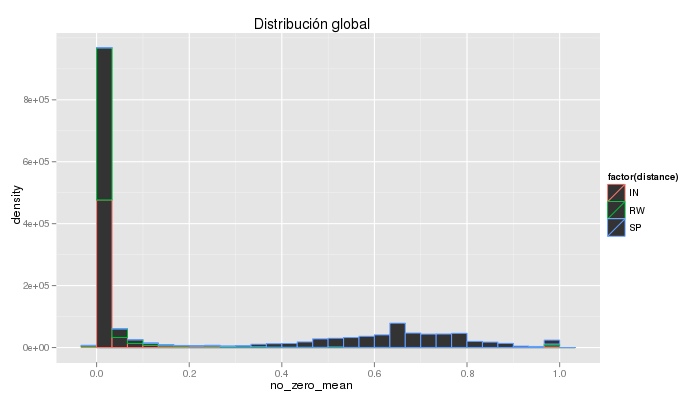
\includegraphics[scale=0.45]{images/emp_tabla_global.png} 
\caption{Distribución global de los estadísticos de priorización obtenidos para el total de simulaciones. La distribución muestra claramente comportamientos muy distintos entre las medidas de distancia planteadas.}
\label{fig:emp_global}
\end{figure}

\medskip
\medskip

\begin{figure}[H]
\centering
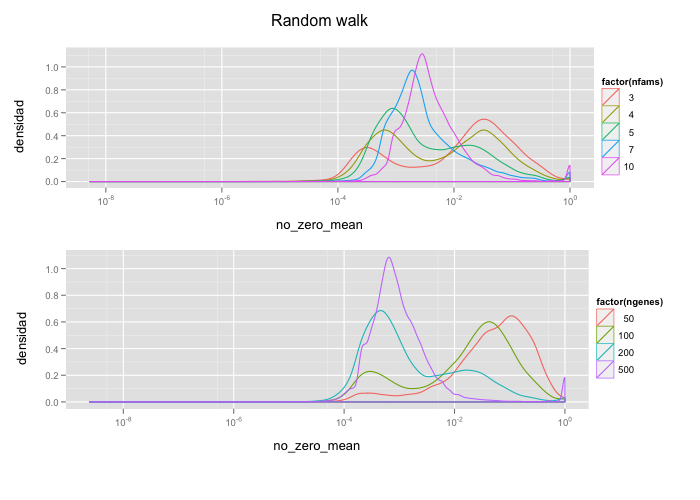
\includegraphics[scale=0.45]{images/emp_rw_nfams_ngenes.png} 
\caption{Distribución global del estadístico de priorización para diferente número de familias (arriba) y diferente número de genes por familia (abajo)..}
\label{fig:emp_rw_nfams_ngenes}
\end{figure}

\medskip
\medskip
 
\subsection{Eficacia en la priorización}

En este apartado, se detallan los resultados obtenidos en las distintas tandas de simulación generadas con el fin de evaluar tanto las medidas de distancia, como la influencia de los parámetros \emph{número de familias}, \emph{número de genes por familia} y \emph{número de genes de enfermedad} sobre los resultados. 

\medskip
Hay que destacar, que en la mayor parte de ocasiones, la fiabilidad de la metodología se ha evaluado a partir de la posición relativa en el ranking de los genes de enfermedad, donde un valor próximo a 1 indicará que han sido convenientemente priorizados por encima del resto de genes aleatorios y que por tanto, la metodología propuesta es efectiva.

\subsubsection{Medidas de distancia}

Las medidas de distancia propuestas han sido evaluadas a partir de las tandas de simulación descritas en la tabla \ref{tab:tabla_distancias} del apartado de material y métodos. Los resultados obtenidos se muestran en la figura \ref{fig:distancias}, la cual representa la posición relativa en el ranking para los genes de enfermedad en las 3 medidas de distancia (\emph{Shortest Path}, intermediación y \emph{Random Walk}) y en los 5 interactomas seleccionados (\emph{binding, functional, ptmod, regulation y textmining}). 

\medskip
Además, se han incluido dos medidas adicionales (\emph{no zero mean} y \emph{no zero max}) correspondientes a las dos funciones propuestas (media y máximo) para proporcionar una medida conjunta de todos los interactomas. Asímismo, las gráficas se han complementado con una barra (de color amarillo) en cada medida, correspondiente a la proporción de genes analizados que no presentan ninguna interacción descrita, y que, por tanto, no han podido ser evaluados en el interactoma correspondiente. 

\begin{figure}[H]
\centering
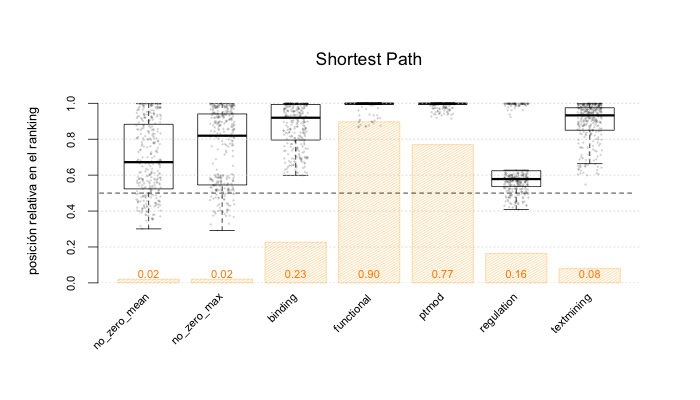
\includegraphics[scale=0.45]{images/sp_summary.png}
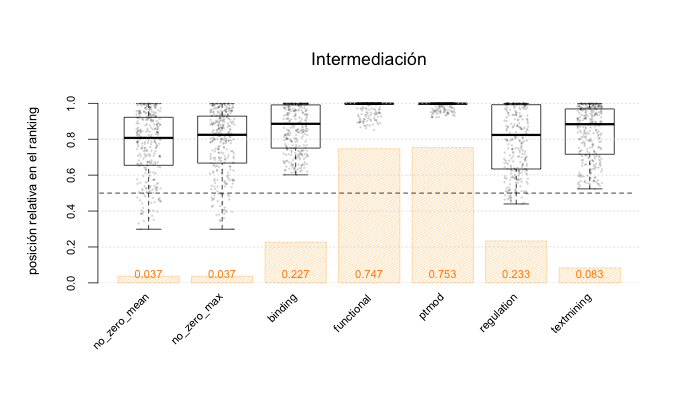
\includegraphics[scale=0.45]{images/inter_summary.png}
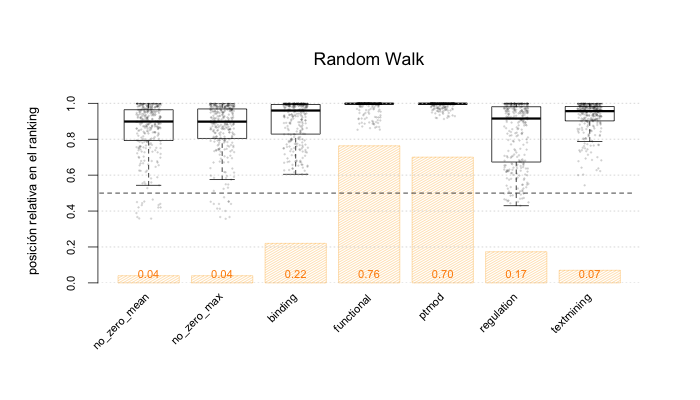
\includegraphics[scale=0.45]{images/rw_summary.png}
\caption{Distribución de la posición relativa en el ranking de los genes de enfermedad para cada medida de distancia \emph{Shortest Path}, intermediación y \emph{Random walk} y cada interactoma. Las barras en amarillo bajo cada interactoma describen la proporción de genes que no han tenido ninguna interacción descrita}
\label{fig:distancias}
\end{figure}

\medskip
Las gráficas describen con claridad como el método \emph{Random walk} proporciona la mejor posición relativa en el ranking para los genes de enfermedad, siendo una mejora perceptible tanto en las medidas por interactoma, como en las medidas globales. Asímismo, se observa que la medida de distancia de intermediación resulta superior a la de \emph{Shortest Path} en todos los casos.

\medskip
En cuanto a los resultados obtenidos por interactoma, se observa claramente que tanto el interactoma funcional, como el de modificaciones post-transduccionales (\emph{functional} y \emph{ptmod} respectivamente) proporcionan con diferencia los mejores resultados, pero también, un porcentaje de genes no descritos muy superior al resto. 

\medskip
A excepción de la medida de distancia \emph{Shortest Path}, tanto la media como el máximo global proporcionan resultados muy similares. Hay que destacar que, salvo el interactoma de regulación, ambas medidas proporcionan un valor de posición en el ranking inferior al de los interactomas, aunque, con un porcentaje de genes no descritos muy inferior al resto.

\subsubsection{Número de familias}

La tabla \ref{tab:tabla_familias} muestra el conjunto de simulaciones planteados para evaluar la influencia del número de familias sobre el resultado. La figura \ref{fig:familias} muestra la distribución de la posición relativa en el ranking para los genes de enfermedad para las 3 medidas de distancia, donde se han usado 3,4,5,7 y 10 familias respectivamente. 

\begin{figure}[H]
\centering
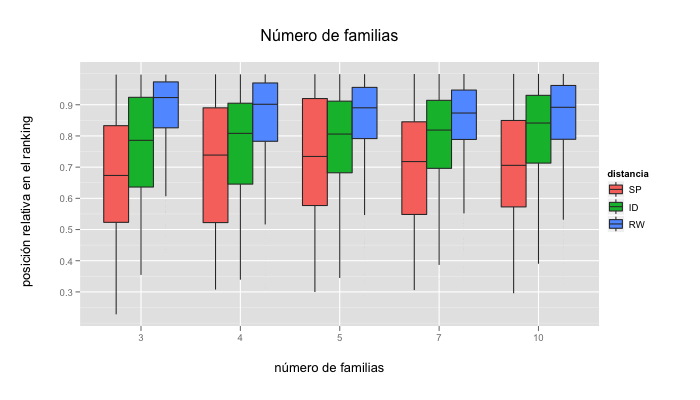
\includegraphics[scale=0.5]{images/tabla_familias.png}
\caption{Distribución de la posición relativa del ranking de los genes de enfermedad para cada número de familias y cada medida de distancia}
\label{fig:familias}
\end{figure}

\medskip
En general, el número de familias no constituye un parámetro que modifique la fiabilidad del resultado. Todas las medidas de distancias muestran  medianas parecidas con dispersión casi constante, siendo la medida de \emph{Shortest Path} la más inestable.
 

\subsubsection{Número de genes por familia}

El número de genes por familia se ha evaluado a partir de las simulaciones planteadas en la tabla \ref{tab:tabla_genes}. La figura \ref{fig:genes} muestra la evolución de la posición relativa en el ranking en función del número de genes por familia.

\begin{figure}[H]
\centering
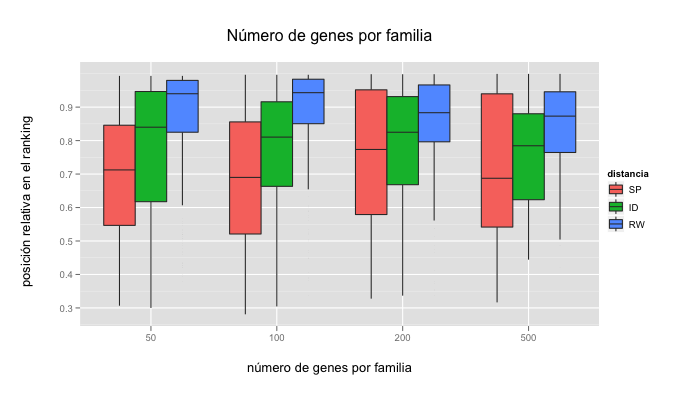
\includegraphics[scale=0.5]{images/tabla_genes.png}
\caption{*****}
\label{fig:genes} 
\end{figure}

\medskip
También en este caso, la medida de \emph{Shortest Path} muestra un comportamiento irregular. Por otro lado, tanto en la distancia de intermediación, como con \emph{Random walk} se aprecia una ligera tendencia decreciente de la mediana, a medida que aumenta el número de genes por familia, con una dispersión casi constante.

\subsubsection{Solapamiento entre familias}

El solapamiento entre familias a nivel de genes de enfermedad se ha evaluado a través de los experimentos planteados en la tabla \ref{tab:tabla_disease}. Todas las simulación se han realizado con 5 familias, donde el número de genes de enfermedad ha estado en el rango de 1 a 5. 

\medskip
La figura \ref{fig:disease} muestra la variación de la posición relativa en el ranking a medida que aumenta el número de genes distintos de enfermedad.

\begin{figure}[H]
\centering
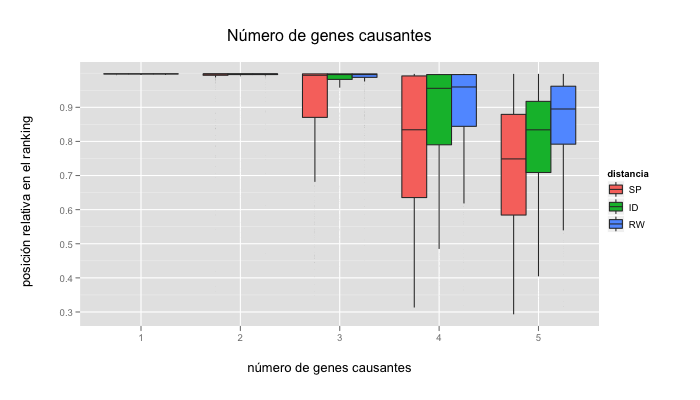
\includegraphics[scale=0.5]{images/tabla_disease.png}
\caption{*****}
\label{fig:disease} 
\end{figure}

\medskip
Tal y como se aprecia, el número de genes de enfermedad distintos tiene una influencia clara sobre el resultado. En aquellos casos donde el número de genes distintos es pequeño, y por tanto, hay gran solapamiento entre familias, se obtienen resultados considerablemente mejores para cualquiera de las medidas de distancia. 

\medskip
También en este caso, \emph{Randow Walk }ofrece los mejores resultados, seguido de la distancia de intermediación.

\section{Caso de uso}

\chapter{Conclusiones}

\section{Validez del método}


\section{Aportación del método en ausencia de genes conocidos}


\section{Limitaciones de la metodología y líneas futuras}


medidas de distancia más óptimas***

interactomas incompletos***
\chapter{Agradecimientos} 


\bibliography{referencias}



\chapter{Material suplementario}

\appendix
\section{First Appendix}


\end{document}